\section{Introduction}
\label{sec:introduction}

A solver that has obtained a candidate answer still has to decide what comes next: repeat the calculation, try another approach, or check the candidate against the original constraints.
%
These choices determine both the quality of the answer and the computation spent reaching it.
%
Longer reasoning can improve performance on demanding problems, but additional steps can also repeat work or extend an unsuccessful search~\citep{chen2025overthinking,muennighoff2025s1}.
%
Efficient reasoning therefore depends on which activities receive computation and when they occur.
%

Large language models (LLMs) with mixture-of-experts (MoE) architectures expose this allocation inside the network.
%
At each sparse layer, a router selects a small subset of feed-forward experts to process the current token~\citep{shazeer2017moe,fedus2022switch}.
%
Changing those selections offers a way to intervene during reasoning while preserving the model weights.
%
The central question is whether routes associated with an activity, such as verification, can help redirect a solution at the point where that activity is useful.
%
Figure~\ref{fig:overview} illustrates the connection between visible reasoning states, expert allocations, and intervention outcomes.
%

\begin{figure}[tb]
\centering
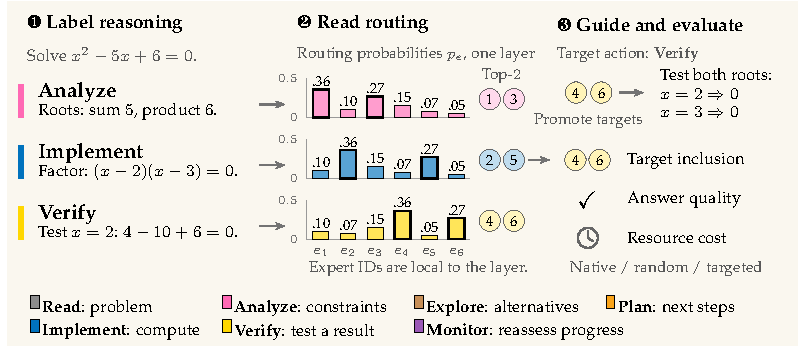
\includegraphics[width=\linewidth]{figures/journal/overview.pdf}
\caption{Reasoning states and routing probabilities in a constructed six-expert example.
%
Dark outlines and circled IDs identify the top-2 experts.
%
The seven-state key connects sentence function to color.
%
Promoting a Verify target set illustrates a checking continuation, whose target engagement, answer quality, and resource cost require separate evaluation.
%
Probabilities and text are explanatory examples, not measured effects.}
\label{fig:overview}
\end{figure}

Existing approaches regulate reasoning length through generation budgets or modify hidden representations to favor particular behaviors~\citep{muennighoff2025s1,chen2025seal,eisenstadt2025overclocking}.
%
Expert steering provides a complementary mechanism by promoting or suppressing behavior-associated experts~\citep{fayyaz2025steermoe}.
%
Online rerouting instead adapts selection scores to the available context~\citep{su2026rewiring}.
%
These approaches establish useful control interfaces, but they do not make every activity-associated route a beneficial intervention.
%
An expert may correlate with checking because it processes characteristic words.
%
Promoting it may change the route without producing a substantive check.
%
Answer quality and computational cost must therefore accompany the behavioral measurement.
%

We study routing interventions through a sequence of connected questions.
%
First, do expert selections contain information about a reasoning state beyond the text that expresses it?
%
Second, how do these states recur and transition, and does routing anticipate the next state?
%
Third, can a state-aware allocation preserve less frequent activities under a limited expert budget?
%
Finally, does activating or deactivating the experts nominated for a state move the reasoning toward or away from that state, and does it shorten the solution at retained accuracy?
%
We use mathematical reasoning as the evaluation setting and analyze eight MoE LLMs with separate controls for these questions.
%
The annotation vocabulary describes the visible function of a sentence.
%
It does not assume that an expert implements a dedicated cognitive operation.
%

Our contributions are the following.
%
\begin{enumerate}
\renewcommand{\labelenumi}{\circnum{\arabic{enumi}}}
\item We connect native expert allocation to interpretable reasoning states using held-out families and text-controlled readouts.
%
Routing adds state information in every analyzed model, supplying a measured basis for investigating state-conditioned interventions.
%
\item We characterize state occupancy, transitions, and duration across the eight models, distinguishing continued execution from returns to a state.
%
The next-state readouts in GPT-OSS and Qwen3.6 test whether routing anticipates a subsequent activity.
%
\item We compare expert retention under a fixed budget, where state balancing improves minimum native coverage in six models and reduces it in two.
%
\item We test state-conditioned routing edits in 29,377 paired continuations from frozen prefixes, with matched random controls and a pre-registered link to native solution length.
%
Activation and deactivation change neither the subsequent reasoning state nor the generated tokens and accuracy beyond matched random edits, although native states such as verification precede shorter remaining reasoning.
%
\end{enumerate}

Routing offers an intervention point within the computation of an LLM.
%
Our results show that it records which reasoning activity is under way, while brief edits to the experts associated with an activity leave the reasoning and its cost unchanged.
%
